% ==========
%  CHƯƠNG 1
% ==========
\OpenGrid

\ParallelChapter
  {Reasoning and Sense Making}
  {Luận và hiểu}
  {}

\TriPara
{
  \EN{\emph{A high school mathematics program based on reasoning and sense making will prepare students for citizenship, for the workplace, and for further study.}}
}
{
  \VI{\emph{Chương trình toán trung học phổ thông dựa trên luận và hiểu sẽ chuẩn bị cho học sinh đảm nhận vai trò công dân, bước vào môi trường lao động và tiếp tục học tập ở bậc sau trung học.}}
}
{
  \NOTE{\emph{Đề từ} đóng vai trò định hướng tư tưởng---toàn bộ nội dung chương được triển khai nhằm làm rõ và luận chứng cho phát biểu này.
  
  Ở đây, luận và hiểu không chỉ thuộc phạm vi nội bộ toán học, mà còn gắn trực tiếp với việc chuẩn bị cho học sinh bước vào đời sống, lao động và học tập.}
}

\TriPara
{
  \EN{High school mathematics prepares students for possible postsecondary work and study in three broad areas (cf. NCTM [2000a]):
  \begin{enumerate}
    \item Mathematics for life
    \item Mathematics for the workplace
    \item Mathematics for the scientific and technical community
  \end{enumerate}    
  As the demands for mathematical literacy increase, students face challenges in all three areas. First, the report of the Programme for International Student Assessment (2007) suggests that students in the United States are lagging in mathematical literacy, which that report defines as the ability to apply mathematics ``to analyse, reason and communicate effectively as they pose, solve and interpret mathematical problems in a variety of situations'' (p. 304), including as future citizens. Second, globalization and the rise of technology are presenting new economic and workforce challenges (Friedman 2007), and the traditional mathematics curriculum is insufficient for students entering many fields (Ganter and Barker 2004). Finally, the United States is in danger of losing its leadership position in science, technology, engineering, and mathematics (Task Force on the Future of American Innovation 2005; Committee on Science, Engineering and Public Policy 2006; Tapping America's Potential 2008).}
}
{
  \VI{Toán trung học phổ thông chuẩn bị cho học sinh làm việc và học tập sau trung học trong ba phương diện lớn (so sánh với NCTM [2000a]):
  \begin{enumerate}
    \item Toán học cho đời sống
    \item Toán học cho môi trường lao động
    \item Toán học cho cộng đồng khoa học và công nghệ
  \end{enumerate}
  Khi yêu cầu về năng lực toán học ngày càng gia tăng, học sinh phải đối mặt với thách thức trong cả ba phương diện này. Thứ nhất, báo cáo của Chương trình Đánh giá Học sinh Quốc tế (PISA) (2007) cho thấy học sinh tại Hoa Kì đang tụt hậu về năng lực toán học. Báo cáo này định nghĩa năng lực toán học là khả năng vận dụng toán học ``để phân tích, luận và giao tiếp hiệu quả khi đặt ra, giải quyết và diễn giải vấn đề toán học trong nhiều tình huống khác nhau'' (p. 304), kể cả với tư cách công dân tương lai. Thứ hai, toàn cầu hóa và sự phát triển của công nghệ đang tạo ra thách thức mới về kinh tế và lực lượng lao động (Friedman 2007), trong khi chương trình toán truyền thống không còn đủ cho học sinh bước vào nhiều lĩnh vực (Ganter and Barker 2004). Cuối cùng, Hoa Kì đang đứng trước nguy cơ đánh mất vị thế dẫn đầu trong khoa học, công nghệ, kĩ thuật và toán học (Task Force on the Future of American Innovation 2005; Committee on Science, Engineering and Public Policy 2006; Tapping America's Potential 2008).}
}
{
  \NOTE{Ba phương diện mà giáo dục toán học trung học phổ thông phải chuẩn bị cho học sinh được nêu rõ: đời sống công dân, môi trường lao động, cùng với cộng đồng khoa học và công nghệ. Cả ba phương diện này đang đồng thời chịu áp lực gia tăng. 

  Dẫn chứng từ PISA cho thấy học sinh đang tụt hậu về năng lực toán học. Theo định nghĩa của PISA, năng lực này là khả năng vận dụng toán học để phân tích, luận, giao tiếp và diễn giải vấn đề trong nhiều tình huống khác nhau, kể cả tình huống gắn với đời sống công dân. Bên cạnh đó, toàn cầu hóa và sự phát triển công nghệ đang làm thay đổi yêu cầu của lực lượng lao động, trong khi chương trình toán truyền thống không còn đủ để đáp ứng nhiều lĩnh vực nghề nghiệp. Ở bình diện rộng hơn, cảnh báo về STEM cho thấy vấn đề này gắn trực tiếp với năng lực khoa học và công nghệ của quốc gia.

  Như vậy, đoạn văn thiết lập một chẩn đoán: nhu cầu xã hội đã thay đổi, nhưng cách tổ chức học tập toán học hiện tại chưa theo kịp.

  \noindent\rule{\linewidth}{0.4pt}

  \noindent\textbf{STEM} là viết tắt của bốn lĩnh vực dưới đây.
  \begin{itemize}
    \item \textbf{S}cience: Khoa học.
    \item \textbf{T}echnology: Công nghệ.
    \item \textbf{E}ngineering: Kĩ thuật.
    \item \textbf{M}athematics: Toán học.
  \end{itemize}
  Nhắc đến STEM nhằm đặt vấn đề giáo dục toán học trong mối liên hệ với yêu cầu phát triển khoa học và công nghệ ở tầm quốc gia.}
}

\TriPara
{
  \EN{A focus on reasoning and sense making, when developed in the context of important content, will ensure that students can accurately carry out mathematical procedures, understand why those procedures work, and know how they might be used and their results interpreted. This understanding will expand students' abilities to apply mathematical perspectives, concepts, and tools flexibly in each of the three areas mentioned above. Such a focus on reasoning and sense making will produce citizens who make informed and reasoned decisions, including quantitatively sophisticated choices about their personal finances, about which public policies deserve their support, and about which insurance or health plans to select. It will also produce workers who can satisfy the increased mathe matical needs in professional areas ranging from health care to small business to digital technology (American Diploma Project 2004).}
}
{
  \VI{Khi được phát triển trong bối cảnh những nội dung quan trọng, việc lấy luận và hiểu làm trọng tâm sẽ bảo đảm rằng học sinh có thể thực hiện chính xác các thủ tục toán học, hiểu vì sao những thủ tục ấy có hiệu lực, và biết chúng có thể được sử dụng như thế nào cũng như kết quả của chúng cần được diễn giải ra sao. Sự hiểu biết đó sẽ mở rộng năng lực của học sinh trong việc vận dụng linh hoạt các góc nhìn, khái niệm và công cụ toán học vào từng phương diện trong ba phương diện nêu trên. Trọng tâm như vậy vào luận và hiểu sẽ tạo nên những công dân có khả năng đưa ra quyết định có căn cứ và có luận cứ, bao gồm những lựa chọn đòi hỏi năng lực định lượng cao về tài chính cá nhân, về chính sách công nào xứng đáng nhận được sự ủng hộ của họ, và về gói bảo hiểm hoặc chăm sóc sức khỏe nào nên được lựa chọn. Nó cũng sẽ tạo nên những người lao động có thể đáp ứng nhu cầu toán học ngày càng gia tăng trong nhiều lĩnh vực nghề nghiệp, từ chăm sóc sức khỏe đến doanh nghiệp nhỏ và công nghệ số (American Diploma Project 2004).}
}
  {\NOTE{}}

\TriPara
{
  \EN{A high school curriculum that focuses on reasoning and sense making will help satisfy the increasing demand for scientists, engineers, and mathematicians while preparing students for whatever professional, vocational, or technical needs may arise. Recent studies suggest that students will experience career changes multiple times during their lives (U.S. Department of Labor 2006), and many of the jobs they will hold in the future do not yet exist. Mathematics is increasingly essential for a wide range of careers, including finance, advertising, forensics, and sports journalism. The advent of the Internet has produced an explosion of new careers in mathematics and statistics that involve harnessing the huge amount of data at people's fingertips (Baker and Leak 2006). By emphasizing both content and reasoning ability, high school mathematics programs can help prepare workers who are able to navigate this uncharted territory.}
}
{
  \VI{Chương trình toán trung học phổ thông lấy luận và hiểu làm trọng tâm sẽ góp phần đáp ứng nhu cầu ngày càng tăng đối với đội ngũ nhà khoa học, kĩ sư và nhà toán học, đồng thời chuẩn bị cho học sinh trước những nhu cầu chuyên môn, nghề nghiệp hoặc kĩ thuật có thể nảy sinh. Các nghiên cứu gần đây cho thấy học sinh sẽ trải qua nhiều lần thay đổi nghề nghiệp trong suốt cuộc đời (U.S. Department of Labor 2006), và nhiều công việc mà các em sẽ đảm nhận trong tương lai hiện nay còn chưa tồn tại. Toán học ngày càng trở nên thiết yếu đối với một phổ nghề nghiệp rộng, bao gồm tài chính, quảng cáo, pháp y và báo chí thể thao. Sự ra đời của Internet đã dẫn tới sự bùng nổ những nghề nghiệp mới trong toán học và thống kê, gắn với việc khai thác khối lượng dữ liệu khổng lồ đang ở ngay trong tầm tay con người (Baker and Leak 2006). Bằng cách đồng thời nhấn mạnh nội dung và năng lực luận, chương trình toán trung học phổ thông có thể góp phần chuẩn bị những người lao động có khả năng định hướng trong miền nghề nghiệp còn chưa có sẵn bản đồ.}
}
{
  \NOTE{Trọng tâm của đoạn này là giá trị chuẩn bị dài hạn của toán học trung học phổ thông. Thế giới nghề nghiệp không đứng yên: người học có thể đổi nghề nhiều lần, và nhiều công việc tương lai còn chưa xuất hiện. Trong bối cảnh ấy, toán học không chỉ phục vụ một số ngành chuyên biệt, mà trở thành năng lực nền cho nhiều lĩnh vực ngày càng gắn với dữ liệu, công nghệ và quyết định định lượng. Vì vậy, việc nhấn mạnh đồng thời nội dung và năng lực luận được trình bày như một cách chuẩn bị cho người học khả năng thích ứng, định hướng và làm việc trong những bối cảnh nghề nghiệp chưa thể dự liệu trọn vẹn.}
}

\ParallelSection
  {What Are Reasoning and Sense Making?}
  {Luận và hiểu là gì?}
  {}

\TriPara
{
  \EN{In the most general terms, reasoning can be thought of as the process of drawing conclusions on the basis of evidence or stated assumptions. Although reasoning is an important part of all disciplines, it plays a special and fundamental role in mathematics. Reasoning in mathematics is often understood to encompass formal reasoning, or proof, in which conclusions are logically deduced from assumptions and definitions. However, mathematical reasoning can take many forms, ranging from informal explanation and justification to formal deduction, as well as inductive observations. Reasoning often begins with explorations, conjectures at various levels, false starts, and partial explanations before a result is reached. As students develop a repertoire of increasingly sophisticated methods of reasoning and proof during their time in high school, ``standards for accepting explanations should become more stringent'' (NCTM 2000a, p. 342).}
}
{
  \VI{Theo nghĩa khái quát nhất, luận có thể được xem là quá trình rút ra kết luận trên cơ sở chứng cứ hoặc giả định đã nêu. Mặc dù luận là phần quan trọng trong mọi ngành học, nó giữ vai trò đặc biệt và nền tảng trong toán học. Trong toán học, luận thường được hiểu là bao hàm luận hình thức, tức chứng minh, trong đó kết luận được suy diễn một cách logic từ giả định và định nghĩa. Tuy nhiên, luận toán học có thể mang nhiều hình thức khác nhau, từ giải thích và biện minh phi hình thức đến suy diễn hình thức, cũng như những quan sát mang tính quy nạp. Luận thường bắt đầu bằng tìm tòi, phỏng đoán ở nhiều cấp độ, khởi đầu sai hướng, và giải thích còn dang dở trước khi đi tới kết quả. Khi học sinh phát triển dần vốn phương pháp luận và chứng minh ngày càng tinh vi trong suốt thời gian học trung học phổ thông, thì ``chuẩn mực chấp nhận lời giải thích cần trở nên nghiêm ngặt hơn'' (NCTM 2000a, p. 342).}
}
{
  \NOTE{
  \noindent\textbf{Luận điểm}\vspace{.25\baselineskip}

  Từ cách mô tả này, có thể thấy vị trí trung tâm của việc học toán không nên chỉ là đáp án hay kĩ thuật giải, mà là quá trình luận dẫn tới đáp án ấy. Những thăm dò, phỏng đoán, sai hướng ban đầu, biện minh từng phần và sự tinh chỉnh lập luận không phải phần phụ bên lề lời giải, mà là nơi học sinh học cách làm toán và dần hình thành năng lực luận.

  Theo nghĩa đó, quá trình luận của học sinh là điểm tựa sư phạm quan trọng mà giáo viên cần tổ chức và khai thác trong lớp học.

  Tuy nhiên, trong thực tế dạy học, điểm tựa này thường bị che khuất khi trọng tâm dồn vào việc truyền thụ tri thức đã hoàn chỉnh và mẹo giải bài tập. Khi đó, học sinh có thể đi đến đáp án đúng mà vẫn không thật sự hiểu vì sao các bước làm ấy là hợp lí.

  Cách tiếp cận mà NCTM đề xuất đòi hỏi sự chuyển dịch rõ rệt: từ việc trình bày sẵn lời giải và lập luận hoàn chỉnh sang việc tổ chức cho học sinh tham gia vào quá trình hình thành, kiểm tra và tinh chỉnh lập luận. Chỉ trong quá trình ấy, học sinh mới có cơ hội hiểu, dần chấp nhận những chuẩn mực luận nghiêm ngặt hơn, và phát triển năng lực luận một cách bền vững. \vspace{.35\baselineskip}

  \noindent\textbf{Phản biện}\vspace{.25\baselineskip}

  Một phản hồi thường gặp là: khi giải bài tập, học sinh vẫn phải nghĩ và chọn bước làm; như vậy chẳng phải các em vẫn đang luận hay sao?

  Nhận định này đúng ở một mức độ nhất định, nhưng chưa đủ.

  Việc giải bài tập theo thủ tục và mẹo đã được cung cấp sẵn chủ yếu đòi hỏi học sinh thi hành những bước đã được vạch trước, chứ chưa buộc các em tham gia vào việc hình thành lập luận.

  Trong trường hợp ấy, học sinh có thể biết phải làm gì để đi đến đáp án, nhưng không nhất thiết hiểu vì sao con đường đó là hợp lí hay vì sao tri thức toán học lại được tổ chức như vậy. Vì thế, hoạt động giải bài tập không tự động dẫn đến sự phát triển năng lực luận theo nghĩa mà NCTM nhấn mạnh, trừ khi giáo viên chủ ý tổ chức cho học sinh tham gia vào việc xây dựng, biện minh và tinh chỉnh lập luận.

  Sơ đồ dưới đây không nhằm chia luận toán học thành hai loại tách biệt, mà chỉ làm rõ hai cách tham gia rất khác nhau của học sinh vào quá trình luận trong lớp học. \vspace{.35\baselineskip}

  \noindent\textbf{Hai cách tham gia vào luận toán học}\vspace{.25\baselineskip}

  \begin{enumerate}
    \item tham gia ở mức thi hành quy trình
      \begin{itemize}
        \item tri thức đầu vào: đã được cho sẵn
          \begin{itemize}
            \item công thức
            \item quy trình
            \item mẹo giải
          \end{itemize}
        \item hoạt động chính của học sinh
          \begin{itemize}
            \item nhận diện dạng bài
            \item áp dụng đúng bước
            \item thao tác chính xác
          \end{itemize}
        \item câu hỏi trung tâm
          \begin{itemize}
            \item dùng công thức nào
          \end{itemize}
        \item hệ quả
          \begin{itemize}
            \item làm được bài quen
            \item sự hiểu dễ mất
            \item khó thích ứng với bài toán mới
          \end{itemize}
      \end{itemize}

    \item tham gia ở mức kiến tạo và biện minh
      \begin{itemize}
        \item tri thức đầu vào: chưa hoàn chỉnh
          \begin{itemize}
            \item tình huống
            \item dữ kiện
            \item vấn đề mở
          \end{itemize}
        \item hoạt động chính của học sinh
          \begin{itemize}
            \item thăm dò, thử--sai
            \item phỏng đoán
            \item biện minh và phản biện
            \item sửa sai và tinh chỉnh
          \end{itemize}
        \item câu hỏi trung tâm
          \begin{itemize}
            \item vì sao cách này hợp lí
          \end{itemize}
        \item hệ quả
          \begin{itemize}
            \item hình thành sự hiểu có cơ sở
            \item phát triển chuẩn mực luận
            \item chuyển tốt sang tình huống mới
          \end{itemize}
      \end{itemize}
  \end{enumerate}

  \noindent\rule{\linewidth}{0.4pt}

  \noindent\textbf{Chú giải ngắn về lựa chọn chuyển ngữ ``luận và hiểu''}\vspace{.25\baselineskip}

  Trong bản dịch này, \emph{reasoning} and \emph{sense making} được chuyển ngữ là ``luận và hiểu''. Theo NCTM, \emph{reasoning} là quá trình đi tới kết luận trên cơ sở chứng cứ hoặc giả định đã nêu; trong toán học, nó không chỉ giới hạn ở chứng minh hay suy diễn hình thức, mà còn bao gồm giải thích, biện minh, quan sát mang tính quy nạp, thăm dò và phỏng đoán. Còn \emph{sense making} là quá trình phát triển sự hiểu về tình huống, bối cảnh hay khái niệm bằng cách nối điều đang xét với tri thức đã có.

  Chữ luận viết là {\hanfont 論}. Các sách chữ Hán giải thích chữ này trước hết theo nghĩa ``bàn nghị'', ``phân tích'', ``nói rõ sự lí''. Vì vậy, luận ở đây không chỉ là nêu ra ý kiến, mà là triển khai và tổ chức lí lẽ để đi tới hoặc bảo vệ kết luận.

  Chữ hiểu được đặt trên nền chữ {\hanfont 曉}. Chữ này vốn có nghĩa gốc là ``sáng'', ``rạng ra'', rồi từ đó mở rộng thành ``biết'', ``hiểu'', ``làm cho rõ''. Vì vậy, hiểu ở đây không chỉ là có thêm mẩu thông tin, mà là chuyển biến nhận thức từ chỗ chưa rõ sang chỗ sáng rõ và thông suốt.

  Theo nghĩa ấy, luận gánh được trục nghĩa của \emph{reasoning}, còn hiểu gánh được trục nghĩa của \emph{sense making}. Chuyển ngữ thành ``luận và hiểu'' vì thế nhằm giữ lại trong tiếng Việt hai chuyển động nhận thức mà văn bản gốc muốn nêu: đi tới kết luận bằng lí lẽ, và làm cho điều đang học trở nên sáng nghĩa.}
}

\TriPara
{
  \EN{We define sense making as developing understanding of a situation, context, or concept by connecting it with existing knowledge. In practice, reasoning and sense making are intertwined across the continuum from informal observations to formal deductions, as seen in figure 1.1, despite the common perception that identifies sense making with the informal end of the continuum and reasoning, especially proof, with the more formal end.}
}
{
  \VI{Chúng tôi định nghĩa hiểu là quá trình làm cho một tình huống, bối cảnh hoặc khái niệm trở nên rõ nghĩa đối với người học bằng cách kết nối điều ấy với tri thức đã có. Trong thực tế, luận và hiểu đan xen với nhau trên một phổ liên tục kéo dài từ quan sát phi hình thức đến suy diễn hình thức, như thể hiện trong Hình 1.1, mặc dù cách nhìn phổ biến thường gắn hiểu với đầu phi hình thức của phổ, còn luận, đặc biệt là chứng minh, với đầu hình thức hơn.}
}
{
  \NOTE{Hiểu trả lời câu hỏi: ``Điều này có nghĩa gì đối với tôi, và nó gắn với điều tôi đã biết như thế nào?''

  Trong khi đó, luận trả lời câu hỏi: ``Từ điều đã chấp nhận, tôi có thể rút ra kết luận nào, và kết luận đó có hợp lí không?''}
}

\TriFigure
  {../figures/fhsm_2009_p4_f1.pdf}
  {../figures/fhsm_2009_p4_f1_vi.pdf}
  {The relationship of reasoning and sense making}
  {Mối liên hệ giữa luận và hiểu}
  {fig: fig_1.1}

\TriPara
{
  \EN{On one hand, formal reasoning may be based on sense making in which one identifies common elements across a number of observations and realizes how those common elements connect with previously experienced situations. On the other hand, ``a good proof is one that also helps one understand the meaning of what is being proved: to see not only that it is true but also why it is true'' (Yackel and Hanna 2003, p.228). As sense making develops, it increasingly incorporates more formal elements. For instance, in example 8, ``Squaring It Away,'' when asked to solve a quadratic equation, students use an informal geometric model to complete the square of the trinomial but then, realizing that more than one solution may exist, they extend the ideas they have developed with more formal algebra to find both solutions.}
}
{
  \VI{Một mặt, luận hình thức có thể dựa trên hiểu, trong đó người học nhận ra yếu tố chung qua nhiều quan sát và nhận thấy cách các yếu tố chung ấy kết nối với những tình huống đã trải nghiệm trước đó. Mặt khác, ``chứng minh tốt là chứng minh cũng giúp ta hiểu ý nghĩa của điều đang được chứng minh: không chỉ thấy rằng điều ấy đúng, mà còn vì sao nó đúng'' (Yackel and Hanna 2003, trang 228). Khi hiểu phát triển, nó ngày càng tích hợp nhiều yếu tố hình thức hơn. Chẳng hạn, trong Ví dụ 8, ``Ổn thỏa bình phương'', khi được yêu cầu giải phương trình bậc hai, học sinh sử dụng mô hình hình học phi hình thức để hoàn thành bình phương của tam thức, nhưng sau đó---khi nhận ra rằng có thể tồn tại nhiều hơn một nghiệm---các em mở rộng những ý tưởng đã hình thành bằng đại số hình thức hơn để tìm cả hai nghiệm.}
}{\NOTE{}}

\TriPara
{
  \EN{Mathematical reasoning and sense making are both important outcomes of mathematics instruction, as well as important means by which students come to know mathematics. As the term is used in this publication, mathematical reasoning encompasses statistical reasoning; see ``Statistical Reasoning'' in chapter 2.}
}
{
  \VI{Luận và hiểu trong toán học vừa là kết quả quan trọng của dạy học toán, vừa là phương tiện quan trọng để học sinh đi đến hiểu biết về toán học. Theo cách dùng trong ấn phẩm này, luận toán học bao hàm cả luận thống kê; xem mục ``Luận thống kê'' trong Chương 2.}
}
{
  \NOTE{Câu này xác lập vai trò kép của luận và hiểu trong dạy học toán. Một mặt, chúng là kết quả cần đạt: sau quá trình học, học sinh không chỉ có thêm tri thức và kĩ thuật, mà còn phải dần có khả năng giải thích, biện minh, kết nối và làm sáng rõ ý tưởng toán học. Mặt khác, chúng cũng là phương tiện của chính việc học: học sinh không đi tới chỗ biết toán bằng cách tiếp nhận thụ động kết quả đã hoàn tất, mà bằng cách tham gia vào quá trình luận và hiểu ngay trong khi học nội dung. Vì vậy, luận và hiểu không phải phần phụ đi sau nội dung, mà là điều vừa cần được hình thành, vừa cần được sử dụng để nội dung toán học trở nên sáng rõ và có thể nắm được. Câu sau đó mở rộng phạm vi của luận toán học theo nghĩa dùng trong ấn phẩm này: nó bao hàm cả luận thống kê, tức không tách việc lí giải trên dữ liệu và bất định ra khỏi khung chung của luận toán học.}
}

\ParallelSection
  {Why Reasoning and Sense Making?}
  {Vì sao cần luận và hiểu?}
  {}

\TriPara
{
  \EN{This publication emphasizes that reasoning and sense making are the foundations of the NCTM Process Standards (2000a). The processes of mathematics---Problem Solving, Reasoning and Proof, Connections, Communication, and Representation---are all manifestations of the act of making sense of mathematics and of reasoning as defined above. Problem solving and proof are impossible without reasoning, and both are avenues through which students develop mathematical reasoning and make sense of mathematical ideas. The communications, connections, and representations chosen by a student must support reasoning and sense making, and reasoning must be employed in making those decisions.}
}
{
  \VI{Ấn phẩm này nhấn mạnh rằng luận và hiểu là nền tảng của các Chuẩn quá trình của NCTM (2000a). Các quá trình toán học---Giải quyết vấn đề, Luận và chứng minh, Kết nối, Giao tiếp, và Biểu diễn---đều là biểu hiện của hoạt động hiểu toán học và hoạt động luận như đã định nghĩa ở trên. Giải quyết vấn đề và chứng minh là không thể thực hiện nếu thiếu luận, và cả hai cũng là con đường để học sinh phát triển luận toán học và hiểu các ý tưởng toán học. Những lựa chọn của học sinh về giao tiếp, kết nối và biểu diễn phải hỗ trợ luận và hiểu; đồng thời, luận cũng phải được vận dụng khi đưa ra các lựa chọn ấy.}
}
{
  \NOTE{Đoạn này khẳng định luận và hiểu không phải chỉ là một chuẩn quá trình bên cạnh các chuẩn khác, mà là nền tảng chung của toàn bộ năm Chuẩn quá trình của NCTM. Giải quyết vấn đề, Luận và chứng minh, Kết nối, Giao tiếp, và Biểu diễn không tồn tại như năm năng lực rời rạc, mà là năm hình thức biểu hiện của luận và hiểu khi được triển khai trong hoạt động toán học.}
}

\TriPara
{
  \EN{Proof is a communication of formal reasoning built on a foundation of sense making, and it is an important outcome of mathematical thinking. Proof can (1) explain why a particular mathematical result must be true, (2) develop autonomous learners by providing the skills needed to evaluate the validity of their own reasoning and that of others, and (3) reveal connections and provide insight into the underlying structure of mathematics (Knuth 2000). Regardless of the specific format of a proof, students may use formal reasoning to make connections with prior learning, extend thinking, support articulation, and stimulate reflection.}
}
{
  \VI{Chứng minh là một hình thức giao tiếp của luận hình thức, được xây dựng trên nền tảng hiểu, đồng thời là kết quả quan trọng của tư duy toán học. Chứng minh có thể (1) giải thích vì sao một kết quả toán học cụ thể phải đúng, (2) phát triển người học tự chủ bằng cách trang bị kĩ năng cần thiết để đánh giá tính hợp lệ trong cách luận của chính mình và của người khác, và (3) làm rõ các kết nối cũng như đem lại cái nhìn vào cấu trúc nền tảng của toán học (Knuth 2000). Bất kể chứng minh được trình bày theo hình thức cụ thể nào, học sinh có thể sử dụng luận hình thức để kết nối với tri thức đã học, mở rộng tư duy, hỗ trợ diễn đạt, và thúc đẩy phản tư.}
}{\NOTE{}}

\TriPara
{
  \EN{At the high school level, reasoning and sense making are of particular importance, but historically ``reasoning'' has been limited to very select areas of the high school curriculum, and sense making is in many instances not present at all. However, an emphasis on students' reasoning and sense making can help students organize their knowledge in ways that enhance the development of number sense, algebraic fluency, functional relationships, geometric reasoning, and statistical thinking, as exemplified in section 2. When students connect new learning with their existing knowledge, they are more likely to understand and retain the new information (Hiebert 2003) than when it is simply presented as a list of isolated procedures. Without such conceptual understanding, “learning new topics becomes harder since there is no network of previously learned concepts and skills to link a new topic to” (Kilpatrick, Swafford, and Findell 2001, p. 123), meaning that procedures may be forgotten as quickly as they are apparently learned. A refocus on reasoning and sense making will increase understanding and foster meaning.}
}
{
  \VI{Ở bậc trung học phổ thông, luận và hiểu có tầm quan trọng đặc biệt; tuy nhiên, xét trong lịch sử, ``luận'' thường chỉ bị giới hạn trong vài mảng rất hẹp của chương trình trung học phổ thông, còn hiểu trong nhiều trường hợp hầu như không hiện diện. Dẫu vậy, việc nhấn mạnh luận và hiểu của học sinh có thể giúp các em tổ chức tri thức theo cách thúc đẩy phát triển cảm thức số, thành thạo đại số, quan hệ hàm số, luận hình học và tư duy thống kê, như được minh họa trong Phần 2. Khi học sinh kết nối điều mới học với tri thức đã có, các em có nhiều khả năng hiểu và ghi nhớ thông tin hơn (Hiebert 2003) so với khi nội dung chỉ được trình bày như danh sách thủ tục rời rạc. Khi thiếu hiểu biết khái niệm như vậy, ``việc học chủ đề mới trở nên khó khăn hơn vì không có mạng lưới khái niệm và kĩ năng đã học trước đó để liên kết với chủ đề mới'' (Kilpatrick, Swafford, and Findell 2001, trang 123), nghĩa là thủ tục có thể bị quên nhanh như lúc tưởng rằng đã học được chúng. Tái tập trung vào luận và hiểu sẽ gia tăng sự hiểu biết và bồi đắp ý nghĩa.}
}{\NOTE{}}

\ParallelSection
  {How Do We Include Reasoning and Sense Making in the Classroom?}
  {Làm thế nào đưa luận và hiểu vào lớp học?}
  {}

\TriPara
{
  \EN{Reasoning and sense making should occur in every mathematics classroom every day. In such an environment, teachers and students ask and answer such questions as ``What's going on here?'' and ``Why do you think that?'' Addressing reasoning and sense making does not need to be an extra burden for teachers struggling with students who are having a difficult time just learning the procedures. On the contrary, the structure that reasoning brings forms a vital support for understanding and continued learning. Currently, many students have difficulty because they find mathematics meaningless. Without the connections that reasoning and sense making provide, a seemingly endless cycle of reteaching may result. With purposeful attention and planning, teachers can hold all students in every high school mathematics classroom accountable for personally engaging in reasoning and sense making, and thus lead students to experience reasoning for themselves rather than merely observe it. Moreover, technology should be used strategically throughout the high school curriculum to help reach this goal; this point is addressed further in chapter 2.}
}
{
  \VI{Luận và hiểu cần diễn ra trong mọi lớp học toán mỗi ngày. Trong môi trường như vậy, giáo viên và học sinh thường xuyên đặt và trả lời câu hỏi như: ``Điều gì đang diễn ra ở đây?'' và ``Vì sao em nghĩ như vậy?''. Việc đưa luận và hiểu vào dạy học không nhất thiết trở thành gánh nặng bổ sung đối với giáo viên đang chật vật với học sinh còn gặp khó khăn ngay cả trong việc học thủ tục. Trái lại, cấu trúc do luận mang lại tạo thành điểm tựa thiết yếu cho sự hiểu và việc học tiếp nối. Hiện nay, nhiều học sinh gặp khó khăn vì thấy toán học không có ý nghĩa. Khi thiếu kết nối do luận và hiểu tạo ra, việc dạy lại có thể rơi vào vòng lặp tưởng như không có hồi kết. Với sự chú ý và chuẩn bị có chủ đích, giáo viên có thể yêu cầu mọi học sinh trong mọi lớp toán trung học phổ thông phải trực tiếp tham gia vào luận và hiểu, từ đó dẫn dắt học sinh tự mình trải nghiệm quá trình luận, thay vì chỉ quan sát người khác luận. Hơn nữa, công nghệ cần được sử dụng một cách chiến lược trong toàn bộ chương trình toán trung học phổ thông để hỗ trợ mục tiêu ấy; vấn đề này sẽ được bàn sâu hơn trong Chương 2.}
}{\NOTE{}}

\TriPara
{
  \EN{What exactly do reasoning and sense making involve in the mathematics classroom? The following example shows how reasoning and sense making can be infused into teaching a formula that many students often regard as meaningless and hard to remember, the distance formula. The first scenario illustrates what frequently happens when students are asked to recall a procedure taught without understanding.}
}
{
  \VI{Cụ thể, luận và hiểu bao gồm những gì trong lớp học toán? Ví dụ sau minh họa cách đưa luận và hiểu vào việc dạy công thức mà nhiều học sinh thường xem là vô nghĩa và khó nhớ: công thức khoảng cách. Kịch bản đầu tiên cho thấy điều thường xảy ra khi học sinh được yêu cầu nhớ lại thủ tục đã được dạy mà không đi kèm sự hiểu.}
}{\NOTE{}}

\TriPara
{
  \EN{
  \begin{scriptlist}
    \item [Teacher:] Today's lesson requires that we calculate the distance between the center of a circle and a point on the circle in order to determine the circle's radius. Who remembers how to find the distance between two points?
    
    \item [Student 1:] Isn't there a formula for that?\vspace{\baselineskip}
    
    \item [Student 2:] I think it's $x_1$ plus $x_2$ squared, or something like that.
    
    \item [Student 1:] Oh, yeah, I remember-there's a great big square root sign, but I don't remember what goes under it.
    
    \item [Student 3:] I know! It's $x_1$ plus $x_2$ all over 2, isn't it?
    
    \item [Student 4:] No, that's the midpoint formula.
  \end{scriptlist}\vspace{\baselineskip}
  (The discussion continues along these lines until the teacher reminds the class of the formula.)}
}
{
  \VI{
  \begin{scriptlist}
    \item[Giáo viên:] Bài học hôm nay yêu cầu chúng ta tính khoảng cách từ tâm đường tròn đến một điểm nằm trên đường tròn để xác định bán kính đường tròn. Ai nhớ cách tìm khoảng cách giữa hai điểm không?
    
    \item[Học sinh 1:] Hình như có công thức cho việc đó thì phải?
    
    \item[Học sinh 2:] Em nghĩ là $x_1$ cộng $x_2$ bình phương, hay gì đó.
    
    \item[Học sinh 1:] À đúng rồi, em nhớ là có dấu căn rất to, nhưng em không nhớ bên dưới là gì.\vspace{\baselineskip}
    
    \item[Học sinh 3:] Em biết! Là $x_1$ cộng $x_2$ rồi chia cho 2, đúng không ạ?
    
    \item[Học sinh 4:] Không, đó là công thức trung điểm.
  \end{scriptlist}
  (Cuộc trao đổi cứ tiếp diễn theo hướng này cho đến khi giáo viên nhắc lại công thức cho cả lớp.)}
}
{
  \NOTE{Kịch bản này là minh họa điển hình cho lớp học trong đó tri thức toán học được tiếp cận như đối tượng để ghi nhớ, chứ không phải để hiểu. Ngay từ câu hỏi mở đầu của giáo viên, trọng tâm đã đặt vào việc ``ai nhớ công thức'', chứ không phải vào việc ``khoảng cách giữa hai điểm là gì'' hay ``vì sao lại cần công thức như vậy''.

  Phản ứng của học sinh cho thấy rõ hệ quả của cách dạy đó. Các em không nói về ý nghĩa hình học của khoảng cách, không liên hệ đến hiểu biết đã có như định lí Pythagoras, mà chỉ cố gắng nhớ lại mảnh kí hiệu rời rạc: có cộng, có bình phương, có dấu căn, có chia. Sự nhầm lẫn giữa công thức khoảng cách và công thức trung điểm không phải lỗi cá nhân của học sinh, mà là hệ quả trực tiếp của việc học công thức như chuỗi kí hiệu có hình thức na ná nhau nhưng không có nền tảng ý nghĩa để phân biệt.

  Cuộc trao đổi trở thành một ``trò chơi đoán công thức'', trong đó cả lớp dò dẫm trí nhớ cho đến khi giáo viên buộc phải can thiệp bằng cách nhắc lại công thức đúng. Khi đó, tri thức không được kiến tạo bởi học sinh mà được trao lại từ giáo viên, củng cố sự phụ thuộc và làm sâu thêm cảm giác rằng toán học là thứ phải nhớ, không phải thứ có thể hiểu.

  Kịch bản này là hình ảnh cụ thể hóa những gì đã được phân tích ở các đoạn trước: khi việc học thiếu luận và hiểu, kiến thức không có cấu trúc, không bám rễ vào hiểu biết, và vì thế dễ quên, dễ nhầm, dễ trở nên vô nghĩa. Công thức không phải vấn đề; vấn đề nằm ở chỗ học sinh không được đặt vào vị thế để hiểu vì sao công thức đó tồn tại. Chính từ bức tranh này, kịch bản tiếp theo sẽ cho thấy cách tiếp cận khác, nơi công thức không còn là thứ phải nhớ, mà là kết quả tự nhiên của quá trình suy nghĩ.}
}

\TriPara
{
  \EN{The next year, this teacher decides to try a different approach that will engage the students in solving a problem. In the following scenario, we see students reasoning about mathematics, connecting what they are learning with their existing knowledge, and making sense of what the distance formula means.}
}
{
  \VI{Năm sau, giáo viên này quyết định thử cách tiếp cận khác, giúp học sinh tham gia giải quyết vấn đề. Trong kịch bản sau, ta thấy học sinh luận về toán học, kết nối điều đang học với tri thức đã có, và hiểu công thức khoảng cách có ý nghĩa gì.}
}{\NOTE{}}

\TriPara
{
  \EN{
  \begin{scriptlist}
  \item[Teacher:] Let's take a look at a situation in which we need to find the distance between two locations on a map. Suppose this map shows your school; your house, which is located two blocks west and five blocks north of school; and your best friend's house, which is located eight blocks east and one block south of school. If the city had a system of evenly spaced perpendicular streets, how many blocks would we have to drive to get from your house to your friend's house?
  
  \item[Student 1:] Well, we would have to drive ten blocks to the east and six blocks to the south, so I guess it would be sixteen blocks, right?
  
  \item[Teacher:] Now, what if you could use a helicopter to fly straight to your friend's house? How could we find the distance ``as the crow flies''? Work with your partners to establish a coordinate-axis system and show the path you'd have to drive to get to your friend's house. Next, work on calculating the direct distance between the houses if you could fly.
  
  \item[Student 1:] What if we use the school as the origin? Then wouldn't my house be at $(-2, 5)$ and my friend's house, at $(8, -1)$?
  
  \item[Student 2:] Yeah, that sounds right. Here, let's draw the path on the streets connecting the two houses and then draw a line segment connecting the two houses.
  
  \item[Student 1:] Maybe we could measure the length of a block and find the distance with a ruler.
  
  \begin{center}
    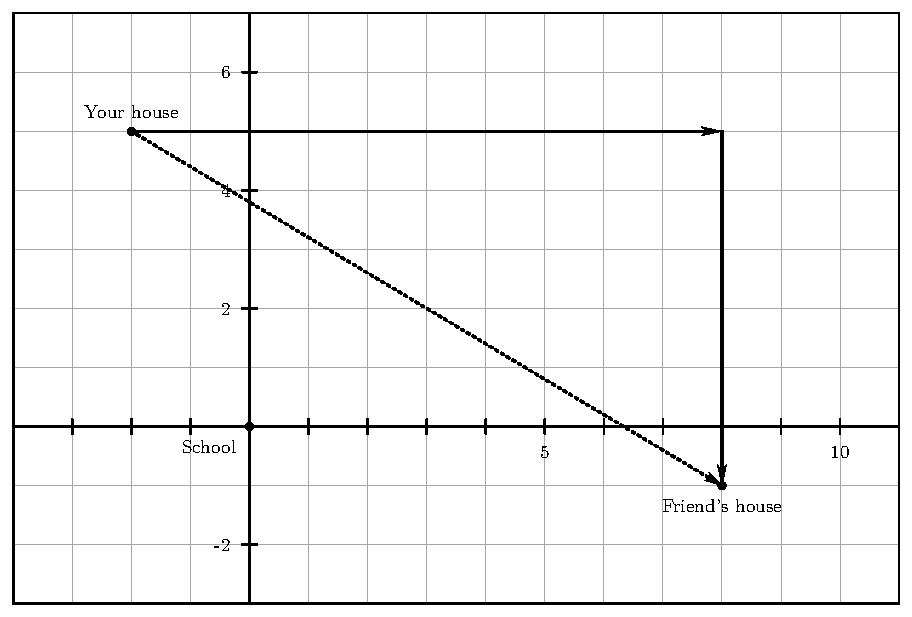
\includegraphics[width=.92\linewidth]{../figures/fhsm_2009_p_7_1.pdf}
  \end{center}

  \item[Student 3:] Wait a minute---you just drew a right triangle, because the streets are perpendicular.
  
  \item[Student 4:] So that means we could use the Pythagorean theorem: $10^2+6^2=c^2$, so $c=\sqrt{136}$.
  
  \item[Student 2:] But how many blocks would that be?
  
  \item[Student 3:] Shouldn't the distance be between eleven and twelve blocks, since $121 < 136 < 144$? Actually, it's probably closer to twelve blocks, since $136$ is much closer to $144$.
  
  (The teacher then extends the discussion to consider other examples and finally to develop a general formula.)
  \end{scriptlist}}
}
{
  \VI{
  \begin{scriptlist}
    \item[Giáo viên:] Hãy xét tình huống cần tìm khoảng cách giữa hai vị trí trên bản đồ. Giả sử bản đồ này thể hiện trường học của em; nhà em nằm cách trường hai dãy phố về phía tây và năm dãy phố về phía bắc, còn nhà bạn thân của em nằm cách trường tám dãy phố về phía đông và một dãy phố về phía nam. Nếu thành phố có hệ thống đường phố vuông góc và cách đều nhau, chúng ta phải đi xe bao nhiêu dãy phố để đi từ nhà em đến nhà bạn em?\vspace{\baselineskip}

    \item[Học sinh 1:] Vậy thì mình phải đi mười dãy phố về phía đông và sáu dãy phố về phía nam, nên chắc là mười sáu dãy phố, đúng không ạ?

    \item[Giáo viên:] Bây giờ, giả sử em có thể dùng trực thăng để bay thẳng đến nhà bạn em. Làm thế nào để tìm được khoảng cách ``đường chim bay''? Hãy làm việc với bạn cùng nhóm để thiết lập hệ trục tọa độ và biểu diễn đường phải đi bằng xe để đến nhà bạn em. Tiếp theo, hãy tính khoảng cách trực tiếp giữa hai ngôi nhà nếu em được bay thẳng.

    \item[Học sinh 1:] Nếu dùng trường học làm gốc tọa độ thì sao ạ? Khi đó, nhà em sẽ ở $(-2, 5)$, còn nhà bạn em ở $(8, -1)$, đúng không?

    \item[Học sinh 2:] Vâng, nghe hợp lí đó. Đây này, hãy vẽ đường đi theo phố nối hai ngôi nhà, rồi vẽ đoạn thẳng nối hai ngôi nhà.\vspace{\baselineskip}

    \item[Học sinh 1:] Có lẽ ta có thể đo chiều dài một dãy phố rồi dùng thước để tìm khoảng cách.
    
      \begin{center}
          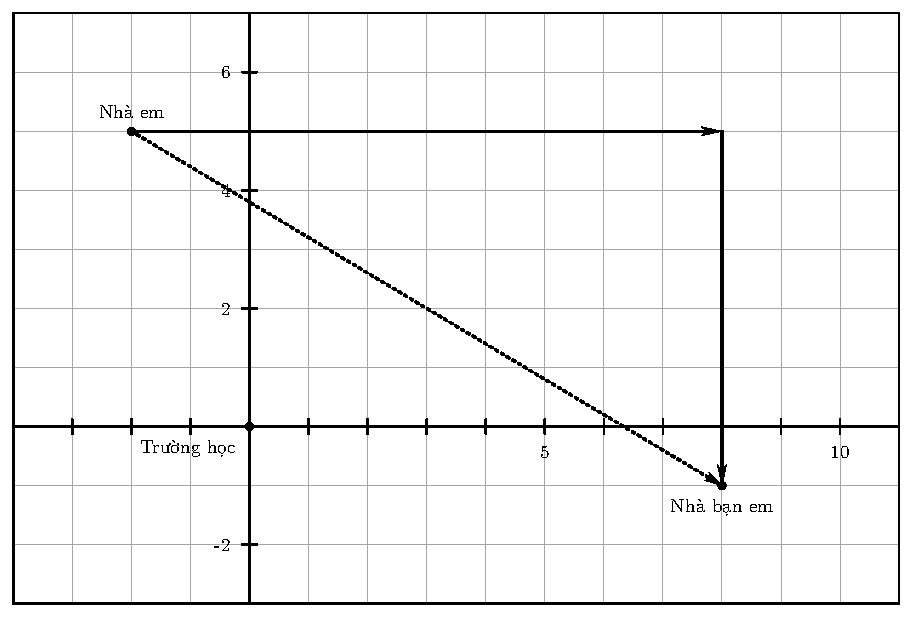
\includegraphics[width=.92\linewidth]{../figures/fhsm_2009_p_7_1_vi.pdf}
      \end{center}

    \item[Học sinh 3:] Khoan đã, bạn vừa vẽ tam giác vuông mà, vì các con phố vuông góc với nhau.

    \item[Học sinh 4:] Vậy nghĩa là ta có thể dùng định lí Pythagoras: $10^2 + 6^2 = c^2$, nên $c = \sqrt{136}$.

    \item[Học sinh 2:] Nhưng như vậy là bao nhiêu dãy phố?

    \item[Học sinh 3:] Chẳng phải khoảng cách phải nằm giữa 11 và 12 dãy phố sao, vì $121 < 136 < 144$? Thực ra, có lẽ nó gần 12 dãy phố hơn, vì $136$ gần $144$ hơn nhiều.\vspace{\baselineskip}
    
    (Sau đó, giáo viên mở rộng thảo luận sang ví dụ khác và cuối cùng xây dựng công thức tổng quát.)
  \end{scriptlist}}
}
{
  \NOTE{Kịch bản này cho thấy lớp học nơi học sinh được đặt vào trung tâm quá trình tư duy toán học, thay vì đứng ngoài quan sát giáo viên trình bày công thức. Điểm xuất phát không phải kí hiệu hay quy trình, mà là tình huống quen thuộc trong đời sống: tìm khoảng cách giữa hai vị trí trên bản đồ thành phố. Chính sự quen thuộc này tạo điều kiện để học sinh bắt đầu hiểu, bởi các em có thể hình dung, ước lượng và dự đoán trước khi đi vào biểu diễn toán học.

  Ở giai đoạn đầu, học sinh tự nhiên đưa ra khoảng cách theo ``đường phố'', tức tổng quãng đường phải đi dọc theo các phố vuông góc. Cách trả lời này không sai, nhưng phản ánh cách hiểu còn gắn với trải nghiệm đời sống. Giáo viên không bác bỏ, mà mở rộng tình huống bằng câu hỏi mới: nếu có thể đi thẳng thì sao? Câu hỏi này buộc học sinh tái cấu trúc vấn đề, từ đó chuyển sang kiểu biểu diễn khác.

  Khi học sinh tự chọn trường học làm gốc tọa độ và xác định vị trí hai ngôi nhà bằng tọa độ, một bước hiểu quan trọng đã diễn ra: các em không chỉ dùng hệ trục tọa độ, mà hiểu vì sao việc đó có ý nghĩa trong tình huống này. Việc vẽ đường đi trên phố và đoạn thẳng nối hai ngôi nhà tạo ra cầu nối trực quan giữa bối cảnh thực và mô hình toán học.

  Khoảnh khắc học sinh nhận ra hình vẽ tạo thành tam giác vuông là bước ngoặt của toàn bộ hoạt động. Ở đây, luận xuất hiện tự nhiên: từ quan sát ``các con phố vuông góc'' đến kết luận ``đây là tam giác vuông'', rồi đến việc vận dụng định lí Pythagoras. Không có công thức nào được nhắc lại từ trí nhớ; thay vào đó, công thức khoảng cách được tái tạo như hệ quả hợp lí của lập luận hình học.

  Đáng chú ý là quá trình này không dừng lại ở tính toán chính xác, mà còn bao gồm suy luận xấp xỉ khi học sinh so sánh 136 với các bình phương lân cận. Điều này cho thấy luận không chỉ là suy luận hình thức, mà còn bao hàm khả năng đánh giá, ước lượng và diễn giải kết quả trong bối cảnh cụ thể.

  Toàn bộ kịch bản minh họa rõ sự khác biệt giữa hai cách dạy: trong kịch bản thứ nhất, học sinh cố gắng nhớ công thức mà không hiểu; trong kịch bản này, công thức xuất hiện như kết quả tự nhiên của chuỗi luận và hiểu đan xen. Kiến thức không còn là thứ được ``trao tay'', mà là thứ được học sinh tự xây dựng thông qua hoạt động tư duy. Chính khác biệt này làm cho công thức khoảng cách trở nên có ý nghĩa, dễ nhớ và có khả năng chuyển giao sang tình huống khác.}
}

\TriPara
{
  \EN{By having her students approach the distance formula from a reasoning-and-sense-making perspective the second year, the teacher increases their understanding of the formula and why it is true, increasing the likelihood that they will be able to retrieve, or quickly recreate, the formula at a later time.}
}
{
  \VI{Khi cho học sinh tiếp cận công thức khoảng cách theo góc nhìn luận và hiểu trong năm thứ hai, giáo viên làm sâu sắc thêm sự hiểu của các em về công thức và lí do công thức đúng, qua đó làm tăng khả năng về sau các em có thể nhớ lại hoặc nhanh chóng tái tạo công thức.}
}{\NOTE{}}

\ParallelSection
  {Conclusion}
  {Kết luận}
  {}

\TriPara
{
  \EN{Reasoning and sense making are the cornerstones of mathematics. Restructuring the high school mathematics program around them enhances students' development of both the content and process knowledge they need to be successful in their continuing study of mathematics and in their lives.}
}
{
  \VI{Luận và hiểu là nền tảng cốt lõi của toán học. Việc tái cấu trúc chương trình toán trung học phổ thông xoay quanh hai nền tảng này sẽ thúc đẩy học sinh phát triển cả tri thức nội dung lẫn tri thức quá trình---những tri thức các em cần để thành công trong việc tiếp tục học toán và trong đời sống.}
}{\NOTE{}}

\CloseGrid